\documentclass[1p]{elsarticle_modified}
%\bibliographystyle{elsarticle-num}

%\usepackage[colorlinks]{hyperref}
%\usepackage{abbrmath_seonhwa} %\Abb, \Ascr, \Acal ,\Abf, \Afrak
\usepackage{amsfonts}
\usepackage{amssymb}
\usepackage{amsmath}
\usepackage{amsthm}
\usepackage{scalefnt}
\usepackage{amsbsy}
\usepackage{kotex}
\usepackage{caption}
\usepackage{subfig}
\usepackage{color}
\usepackage{graphicx}
\usepackage{xcolor} %% white, black, red, green, blue, cyan, magenta, yellow
\usepackage{float}
\usepackage{setspace}
\usepackage{hyperref}

\usepackage{tikz}
\usetikzlibrary{arrows}

\usepackage{multirow}
\usepackage{array} % fixed length table
\usepackage{hhline}

%%%%%%%%%%%%%%%%%%%%%
\makeatletter
\renewcommand*\env@matrix[1][\arraystretch]{%
	\edef\arraystretch{#1}%
	\hskip -\arraycolsep
	\let\@ifnextchar\new@ifnextchar
	\array{*\c@MaxMatrixCols c}}
\makeatother %https://tex.stackexchange.com/questions/14071/how-can-i-increase-the-line-spacing-in-a-matrix
%%%%%%%%%%%%%%%

\usepackage[normalem]{ulem}

\newcommand{\msout}[1]{\ifmmode\text{\sout{\ensuremath{#1}}}\else\sout{#1}\fi}
%SOURCE: \msout is \stkout macro in https://tex.stackexchange.com/questions/20609/strikeout-in-math-mode

\newcommand{\cancel}[1]{
	\ifmmode
	{\color{red}\msout{#1}}
	\else
	{\color{red}\sout{#1}}
	\fi
}

\newcommand{\add}[1]{
	{\color{blue}\uwave{#1}}
}

\newcommand{\replace}[2]{
	\ifmmode
	{\color{red}\msout{#1}}{\color{blue}\uwave{#2}}
	\else
	{\color{red}\sout{#1}}{\color{blue}\uwave{#2}}
	\fi
}

\newcommand{\Sol}{\mathcal{S}} %segment
\newcommand{\D}{D} %diagram
\newcommand{\A}{\mathcal{A}} %arc


%%%%%%%%%%%%%%%%%%%%%%%%%%%%%5 test

\def\sl{\operatorname{\textup{SL}}(2,\Cbb)}
\def\psl{\operatorname{\textup{PSL}}(2,\Cbb)}
\def\quan{\mkern 1mu \triangleright \mkern 1mu}

\theoremstyle{definition}
\newtheorem{thm}{Theorem}[section]
\newtheorem{prop}[thm]{Proposition}
\newtheorem{lem}[thm]{Lemma}
\newtheorem{ques}[thm]{Question}
\newtheorem{cor}[thm]{Corollary}
\newtheorem{defn}[thm]{Definition}
\newtheorem{exam}[thm]{Example}
\newtheorem{rmk}[thm]{Remark}
\newtheorem{alg}[thm]{Algorithm}

\newcommand{\I}{\sqrt{-1}}
\begin{document}

%\begin{frontmatter}
%
%\title{Boundary parabolic representations of knots up to 8 crossings}
%
%%% Group authors per affiliation:
%\author{Yunhi Cho} 
%\address{Department of Mathematics, University of Seoul, Seoul, Korea}
%\ead{yhcho@uos.ac.kr}
%
%
%\author{Seonhwa Kim} %\fnref{s_kim}}
%\address{Center for Geometry and Physics, Institute for Basic Science, Pohang, 37673, Korea}
%\ead{ryeona17@ibs.re.kr}
%
%\author{Hyuk Kim}
%\address{Department of Mathematical Sciences, Seoul National University, Seoul 08826, Korea}
%\ead{hyukkim@snu.ac.kr}
%
%\author{Seokbeom Yoon}
%\address{Department of Mathematical Sciences, Seoul National University, Seoul, 08826,  Korea}
%\ead{sbyoon15@snu.ac.kr}
%
%\begin{abstract}
%We find all boundary parabolic representation of knots up to 8 crossings.
%
%\end{abstract}
%\begin{keyword}
%    \MSC[2010] 57M25 
%\end{keyword}
%
%\end{frontmatter}

%\linenumbers
%\tableofcontents
%
\newcommand\colored[1]{\textcolor{white}{\rule[-0.35ex]{0.8em}{1.4ex}}\kern-0.8em\color{red} #1}%
%\newcommand\colored[1]{\textcolor{white}{ #1}\kern-2.17ex	\textcolor{white}{ #1}\kern-1.81ex	\textcolor{white}{ #1}\kern-2.15ex\color{red}#1	}

{\Large $\underline{12n_{0083}~(K12n_{0083})}$}

\setlength{\tabcolsep}{10pt}
\renewcommand{\arraystretch}{1.6}
\vspace{1cm}\begin{tabular}{m{100pt}>{\centering\arraybackslash}m{274pt}}
\multirow{5}{120pt}{
	\centering
	\includegraphics[width=112pt]{../../../GIT/diagram.site/Diagrams/png/2172_12n_0083.png}\\
\ \ \ A knot diagram\footnotemark}&
\allowdisplaybreaks
\textbf{Linearized knot diagam} \\
\cline{2-2}
 &
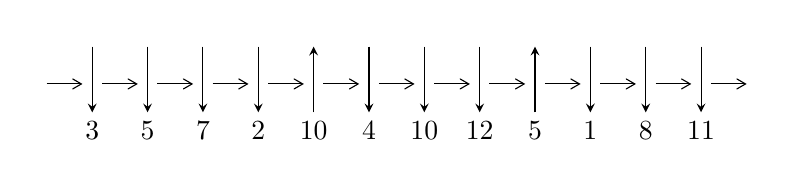
\begin{tikzpicture}[x=20pt, y=17pt]
	% nodes
	\node (C0) at (0, 0) {};
	\node (C1) at (1, 0) {};
	\node (C1U) at (1, +1) {};
	\node (C1D) at (1, -1) {3};

	\node (C2) at (2, 0) {};
	\node (C2U) at (2, +1) {};
	\node (C2D) at (2, -1) {5};

	\node (C3) at (3, 0) {};
	\node (C3U) at (3, +1) {};
	\node (C3D) at (3, -1) {7};

	\node (C4) at (4, 0) {};
	\node (C4U) at (4, +1) {};
	\node (C4D) at (4, -1) {2};

	\node (C5) at (5, 0) {};
	\node (C5U) at (5, +1) {};
	\node (C5D) at (5, -1) {10};

	\node (C6) at (6, 0) {};
	\node (C6U) at (6, +1) {};
	\node (C6D) at (6, -1) {4};

	\node (C7) at (7, 0) {};
	\node (C7U) at (7, +1) {};
	\node (C7D) at (7, -1) {10};

	\node (C8) at (8, 0) {};
	\node (C8U) at (8, +1) {};
	\node (C8D) at (8, -1) {12};

	\node (C9) at (9, 0) {};
	\node (C9U) at (9, +1) {};
	\node (C9D) at (9, -1) {5};

	\node (C10) at (10, 0) {};
	\node (C10U) at (10, +1) {};
	\node (C10D) at (10, -1) {1};

	\node (C11) at (11, 0) {};
	\node (C11U) at (11, +1) {};
	\node (C11D) at (11, -1) {8};

	\node (C12) at (12, 0) {};
	\node (C12U) at (12, +1) {};
	\node (C12D) at (12, -1) {11};
	\node (C13) at (13, 0) {};

	% arrows
	\draw[->,>={angle 60}]
	(C0) edge (C1) (C1) edge (C2) (C2) edge (C3) (C3) edge (C4) (C4) edge (C5) (C5) edge (C6) (C6) edge (C7) (C7) edge (C8) (C8) edge (C9) (C9) edge (C10) (C10) edge (C11) (C11) edge (C12) (C12) edge (C13) ;	\draw[->,>=stealth]
	(C1U) edge (C1D) (C2U) edge (C2D) (C3U) edge (C3D) (C4U) edge (C4D) (C5D) edge (C5U) (C6U) edge (C6D) (C7U) edge (C7D) (C8U) edge (C8D) (C9D) edge (C9U) (C10U) edge (C10D) (C11U) edge (C11D) (C12U) edge (C12D) ;
	\end{tikzpicture} \\
\hhline{~~} \\& 
\textbf{Solving Sequence} \\ \cline{2-2} 
 &
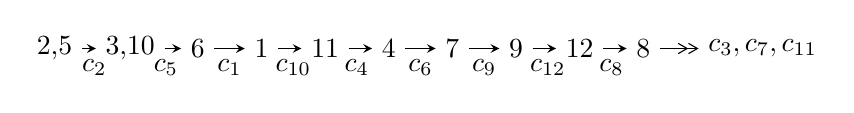
\begin{tikzpicture}[x=23pt, y=7pt]
	% node
	\node (A0) at (-1/8, 0) {2,5};
	\node (A1) at (17/16, 0) {3,10};
	\node (A2) at (17/8, 0) {6};
	\node (A3) at (25/8, 0) {1};
	\node (A4) at (33/8, 0) {11};
	\node (A5) at (41/8, 0) {4};
	\node (A6) at (49/8, 0) {7};
	\node (A7) at (57/8, 0) {9};
	\node (A8) at (65/8, 0) {12};
	\node (A9) at (73/8, 0) {8};
	\node (C1) at (1/2, -1) {$c_{2}$};
	\node (C2) at (13/8, -1) {$c_{5}$};
	\node (C3) at (21/8, -1) {$c_{1}$};
	\node (C4) at (29/8, -1) {$c_{10}$};
	\node (C5) at (37/8, -1) {$c_{4}$};
	\node (C6) at (45/8, -1) {$c_{6}$};
	\node (C7) at (53/8, -1) {$c_{9}$};
	\node (C8) at (61/8, -1) {$c_{12}$};
	\node (C9) at (69/8, -1) {$c_{8}$};
	\node (A10) at (11, 0) {$c_{3},c_{7},c_{11}$};

	% edge
	\draw[->,>=stealth]	
	(A0) edge (A1) (A1) edge (A2) (A2) edge (A3) (A3) edge (A4) (A4) edge (A5) (A5) edge (A6) (A6) edge (A7) (A7) edge (A8) (A8) edge (A9) ;
	\draw[->>,>={angle 60}]	
	(A9) edge (A10);
\end{tikzpicture} \\ 

\end{tabular} \\

\footnotetext{
The image of knot diagram is generated by the software ``\textbf{Draw programme}" developed by Andrew Bartholomew(\url{http://www.layer8.co.uk/maths/draw/index.htm\#Running-draw}), where we modified some parts for our purpose(\url{https://github.com/CATsTAILs/LinksPainter}).
}\phantom \\ \newline 
\centering \textbf{Ideals for irreducible components\footnotemark of $X_{\text{par}}$} 
 
\begin{align*}
I^u_{1}&=\langle 
-7.39937\times10^{54} u^{61}-7.95828\times10^{55} u^{60}+\cdots+9.36658\times10^{54} b+4.21903\times10^{55},\\
\phantom{I^u_{1}}&\phantom{= \langle  }-4.20292\times10^{54} u^{61}-2.34926\times10^{55} u^{60}+\cdots+4.68329\times10^{54} a+1.31817\times10^{55},\;u^{62}+5 u^{61}+\cdots-7 u+1\rangle \\
I^u_{2}&=\langle 
u^2+b+u,\;a,\;u^3+u^2-1\rangle \\
I^u_{3}&=\langle 
b^2+3 u^2+b+5 u+4,\;a,\;u^3+u^2-1\rangle \\
I^u_{4}&=\langle 
b,\;a+1,\;u-1\rangle \\
\\
\end{align*}
\raggedright * 4 irreducible components of $\dim_{\mathbb{C}}=0$, with total 72 representations.\\
\footnotetext{All coefficients of polynomials are rational numbers. But the coefficients are sometimes approximated in decimal forms when there is not enough margin.}
\newpage
\renewcommand{\arraystretch}{1}
\centering \section*{I. $I^u_{1}= \langle -7.40\times10^{54} u^{61}-7.96\times10^{55} u^{60}+\cdots+9.37\times10^{54} b+4.22\times10^{55},\;-4.20\times10^{54} u^{61}-2.35\times10^{55} u^{60}+\cdots+4.68\times10^{54} a+1.32\times10^{55},\;u^{62}+5 u^{61}+\cdots-7 u+1 \rangle$}
\flushleft \textbf{(i) Arc colorings}\\
\begin{tabular}{m{7pt} m{180pt} m{7pt} m{180pt} }
\flushright $a_{2}=$&$\begin{pmatrix}1\\0\end{pmatrix}$ \\
\flushright $a_{5}=$&$\begin{pmatrix}0\\u\end{pmatrix}$ \\
\flushright $a_{3}=$&$\begin{pmatrix}1\\u^2\end{pmatrix}$ \\
\flushright $a_{10}=$&$\begin{pmatrix}0.897429 u^{61}+5.01625 u^{60}+\cdots-31.2394 u-2.81463\\0.789976 u^{61}+8.49647 u^{60}+\cdots+33.8636 u-4.50435\end{pmatrix}$ \\
\flushright $a_{6}=$&$\begin{pmatrix}0.284554 u^{61}+1.83768 u^{60}+\cdots-2.18948 u+3.46404\\-0.353321 u^{61}-0.129700 u^{60}+\cdots-1.33250 u-0.387951\end{pmatrix}$ \\
\flushright $a_{1}=$&$\begin{pmatrix}- u^2+1\\- u^4\end{pmatrix}$ \\
\flushright $a_{11}=$&$\begin{pmatrix}0.873580 u^{61}+3.94211 u^{60}+\cdots-25.2656 u-4.12853\\1.29842 u^{61}+10.9238 u^{60}+\cdots+41.7471 u-5.56745\end{pmatrix}$ \\
\flushright $a_{4}=$&$\begin{pmatrix}u\\u\end{pmatrix}$ \\
\flushright $a_{7}=$&$\begin{pmatrix}0.834045 u^{61}+3.97405 u^{60}+\cdots-11.3813 u+4.68603\\0.196170 u^{61}+2.00667 u^{60}+\cdots-10.5243 u+0.834045\end{pmatrix}$ \\
\flushright $a_{9}=$&$\begin{pmatrix}0.897429 u^{61}+5.01625 u^{60}+\cdots-31.2394 u-2.81463\\0.271747 u^{61}+6.65168 u^{60}+\cdots+36.6699 u-5.03346\end{pmatrix}$ \\
\flushright $a_{12}=$&$\begin{pmatrix}-0.835301 u^{61}-3.12639 u^{60}+\cdots+14.5834 u+4.37470\\-5.11158 u^{61}-24.5806 u^{60}+\cdots-4.66960 u+0.596938\end{pmatrix}$ \\
\flushright $a_{8}=$&$\begin{pmatrix}u^2-1\\2.88576 u^{61}+15.7183 u^{60}+\cdots+14.2886 u-2.18510\end{pmatrix}$\\&\end{tabular}
\flushleft \textbf{(ii) Obstruction class $= -1$}\\~\\
\flushleft \textbf{(iii) Cusp Shapes $= 6.52357 u^{61}+48.3926 u^{60}+\cdots+104.147 u-23.8150$}\\~\\
\newpage\renewcommand{\arraystretch}{1}
\flushleft \textbf{(iv) u-Polynomials at the component}\newline \\
\begin{tabular}{m{50pt}|m{274pt}}
Crossings & \hspace{64pt}u-Polynomials at each crossing \\
\hline $$\begin{aligned}c_{1}\end{aligned}$$&$\begin{aligned}
&u^{62}+35 u^{61}+\cdots+141 u+1
\end{aligned}$\\
\hline $$\begin{aligned}c_{2},c_{4}\end{aligned}$$&$\begin{aligned}
&u^{62}-5 u^{61}+\cdots+7 u+1
\end{aligned}$\\
\hline $$\begin{aligned}c_{3},c_{6}\end{aligned}$$&$\begin{aligned}
&u^{62}-4 u^{61}+\cdots+10 u-2
\end{aligned}$\\
\hline $$\begin{aligned}c_{5},c_{9}\end{aligned}$$&$\begin{aligned}
&u^{62}+4 u^{61}+\cdots+512 u+512
\end{aligned}$\\
\hline $$\begin{aligned}c_{7}\end{aligned}$$&$\begin{aligned}
&u^{62}-3 u^{61}+\cdots+26312 u-2116
\end{aligned}$\\
\hline $$\begin{aligned}c_{8},c_{11}\end{aligned}$$&$\begin{aligned}
&u^{62}+5 u^{61}+\cdots+11 u-1
\end{aligned}$\\
\hline $$\begin{aligned}c_{10},c_{12}\end{aligned}$$&$\begin{aligned}
&u^{62}+23 u^{61}+\cdots+261 u+1
\end{aligned}$\\
\hline
\end{tabular}\\~\\
\newpage\renewcommand{\arraystretch}{1}
\flushleft \textbf{(v) Riley Polynomials at the component}\newline \\
\begin{tabular}{m{50pt}|m{274pt}}
Crossings & \hspace{64pt}Riley Polynomials at each crossing \\
\hline $$\begin{aligned}c_{1}\end{aligned}$$&$\begin{aligned}
&y^{62}-11 y^{61}+\cdots-18829 y+1
\end{aligned}$\\
\hline $$\begin{aligned}c_{2},c_{4}\end{aligned}$$&$\begin{aligned}
&y^{62}-35 y^{61}+\cdots-141 y+1
\end{aligned}$\\
\hline $$\begin{aligned}c_{3},c_{6}\end{aligned}$$&$\begin{aligned}
&y^{62}+18 y^{61}+\cdots-459 y^2+4
\end{aligned}$\\
\hline $$\begin{aligned}c_{5},c_{9}\end{aligned}$$&$\begin{aligned}
&y^{62}+48 y^{61}+\cdots+1703936 y+262144
\end{aligned}$\\
\hline $$\begin{aligned}c_{7}\end{aligned}$$&$\begin{aligned}
&y^{62}-47 y^{61}+\cdots-1209188200 y+4477456
\end{aligned}$\\
\hline $$\begin{aligned}c_{8},c_{11}\end{aligned}$$&$\begin{aligned}
&y^{62}-23 y^{61}+\cdots-261 y+1
\end{aligned}$\\
\hline $$\begin{aligned}c_{10},c_{12}\end{aligned}$$&$\begin{aligned}
&y^{62}+37 y^{61}+\cdots-59949 y+1
\end{aligned}$\\
\hline
\end{tabular}\\~\\
\newpage\flushleft \textbf{(vi) Complex Volumes and Cusp Shapes}
$$\begin{array}{c|c|c}  
\text{Solutions to }I^u_{1}& \I (\text{vol} + \sqrt{-1}CS) & \text{Cusp shape}\\
 \hline 
\begin{aligned}
u &= -0.174819 + 1.015820 I \\
a &= \phantom{-}1.39308 + 0.32509 I \\
b &= -0.169145 + 0.123365 I\end{aligned}
 & -0.70247 - 10.05410 I & -8.00000 + 0. I\phantom{ +0.000000I} \\ \hline\begin{aligned}
u &= -0.174819 - 1.015820 I \\
a &= \phantom{-}1.39308 - 0.32509 I \\
b &= -0.169145 - 0.123365 I\end{aligned}
 & -0.70247 + 10.05410 I & -8.00000 + 0. I\phantom{ +0.000000I} \\ \hline\begin{aligned}
u &= -0.180060 + 0.947177 I \\
a &= -1.40332 - 0.28966 I \\
b &= \phantom{-}0.218716 - 0.044373 I\end{aligned}
 & \phantom{-}0.58990 - 4.34695 I & -4.42907 + 2.23582 I \\ \hline\begin{aligned}
u &= -0.180060 - 0.947177 I \\
a &= -1.40332 + 0.28966 I \\
b &= \phantom{-}0.218716 + 0.044373 I\end{aligned}
 & \phantom{-}0.58990 + 4.34695 I & -4.42907 - 2.23582 I \\ \hline\begin{aligned}
u &= \phantom{-}0.008820 + 0.960888 I \\
a &= \phantom{-}1.46292 + 0.33775 I \\
b &= -0.0127547 - 0.0398138 I\end{aligned}
 & -5.70261 - 3.52968 I & -11.39023 + 3.16583 I \\ \hline\begin{aligned}
u &= \phantom{-}0.008820 - 0.960888 I \\
a &= \phantom{-}1.46292 - 0.33775 I \\
b &= -0.0127547 + 0.0398138 I\end{aligned}
 & -5.70261 + 3.52968 I & -11.39023 - 3.16583 I \\ \hline\begin{aligned}
u &= -0.925664 + 0.154080 I \\
a &= \phantom{-}1.55623 + 0.95238 I \\
b &= \phantom{-}1.16403 + 0.90014 I\end{aligned}
 & -3.09925 + 0.70693 I & -5.36300 - 9.97003 I \\ \hline\begin{aligned}
u &= -0.925664 - 0.154080 I \\
a &= \phantom{-}1.55623 - 0.95238 I \\
b &= \phantom{-}1.16403 - 0.90014 I\end{aligned}
 & -3.09925 - 0.70693 I & -5.36300 + 9.97003 I \\ \hline\begin{aligned}
u &= -0.961954 + 0.456687 I \\
a &= -0.996485 - 0.482853 I \\
b &= -0.773429 - 0.351449 I\end{aligned}
 & \phantom{-}1.77868 + 2.87670 I & \phantom{-0.000000 } 0 \\ \hline\begin{aligned}
u &= -0.961954 - 0.456687 I \\
a &= -0.996485 + 0.482853 I \\
b &= -0.773429 + 0.351449 I\end{aligned}
 & \phantom{-}1.77868 - 2.87670 I & \phantom{-0.000000 } 0\\
 \hline 
 \end{array}$$\newpage$$\begin{array}{c|c|c}  
\text{Solutions to }I^u_{1}& \I (\text{vol} + \sqrt{-1}CS) & \text{Cusp shape}\\
 \hline 
\begin{aligned}
u &= \phantom{-}1.072360 + 0.027388 I \\
a &= \phantom{-}0.302091 + 0.387550 I \\
b &= -0.44401 + 2.52455 I\end{aligned}
 & -2.88487 - 0.32439 I & \phantom{-0.000000 } 0 \\ \hline\begin{aligned}
u &= \phantom{-}1.072360 - 0.027388 I \\
a &= \phantom{-}0.302091 - 0.387550 I \\
b &= -0.44401 - 2.52455 I\end{aligned}
 & -2.88487 + 0.32439 I & \phantom{-0.000000 } 0 \\ \hline\begin{aligned}
u &= \phantom{-}1.026130 + 0.340287 I \\
a &= -0.816921 + 0.074019 I \\
b &= \phantom{-}0.010122 + 1.005580 I\end{aligned}
 & -0.058930 + 1.340430 I & \phantom{-0.000000 } 0 \\ \hline\begin{aligned}
u &= \phantom{-}1.026130 - 0.340287 I \\
a &= -0.816921 - 0.074019 I \\
b &= \phantom{-}0.010122 - 1.005580 I\end{aligned}
 & -0.058930 - 1.340430 I & \phantom{-0.000000 } 0 \\ \hline\begin{aligned}
u &= \phantom{-}0.263341 + 0.858285 I \\
a &= \phantom{-}1.45496 + 0.37428 I \\
b &= \phantom{-}0.129842 - 0.231061 I\end{aligned}
 & -2.48962 + 3.11257 I & -8.69664 - 2.35415 I \\ \hline\begin{aligned}
u &= \phantom{-}0.263341 - 0.858285 I \\
a &= \phantom{-}1.45496 - 0.37428 I \\
b &= \phantom{-}0.129842 + 0.231061 I\end{aligned}
 & -2.48962 - 3.11257 I & -8.69664 + 2.35415 I \\ \hline\begin{aligned}
u &= -0.799508 + 0.362955 I \\
a &= \phantom{-}0.895892 - 0.982033 I \\
b &= -0.36497 - 1.79872 I\end{aligned}
 & \phantom{-}3.99898 + 4.77294 I & -4.23166 - 6.20197 I \\ \hline\begin{aligned}
u &= -0.799508 - 0.362955 I \\
a &= \phantom{-}0.895892 + 0.982033 I \\
b &= -0.36497 + 1.79872 I\end{aligned}
 & \phantom{-}3.99898 - 4.77294 I & -4.23166 + 6.20197 I \\ \hline\begin{aligned}
u &= \phantom{-}0.871772 + 0.018873 I \\
a &= -0.012598 + 0.371703 I \\
b &= \phantom{-}0.29638 + 4.67077 I\end{aligned}
 & \phantom{-}1.75714 - 2.86066 I & -51.0320 + 5.8085 I \\ \hline\begin{aligned}
u &= \phantom{-}0.871772 - 0.018873 I \\
a &= -0.012598 - 0.371703 I \\
b &= \phantom{-}0.29638 - 4.67077 I\end{aligned}
 & \phantom{-}1.75714 + 2.86066 I & -51.0320 - 5.8085 I\\
 \hline 
 \end{array}$$\newpage$$\begin{array}{c|c|c}  
\text{Solutions to }I^u_{1}& \I (\text{vol} + \sqrt{-1}CS) & \text{Cusp shape}\\
 \hline 
\begin{aligned}
u &= -0.896158 + 0.689044 I \\
a &= -0.409815 - 0.214201 I \\
b &= -0.330845 - 0.132174 I\end{aligned}
 & \phantom{-}2.20517 + 2.65821 I & \phantom{-0.000000 } 0 \\ \hline\begin{aligned}
u &= -0.896158 - 0.689044 I \\
a &= -0.409815 + 0.214201 I \\
b &= -0.330845 + 0.132174 I\end{aligned}
 & \phantom{-}2.20517 - 2.65821 I & \phantom{-0.000000 } 0 \\ \hline\begin{aligned}
u &= \phantom{-}1.129020 + 0.261697 I \\
a &= \phantom{-}0.757928 - 0.225431 I \\
b &= -0.024907 - 1.263230 I\end{aligned}
 & -0.33332 - 3.49089 I & \phantom{-0.000000 } 0 \\ \hline\begin{aligned}
u &= \phantom{-}1.129020 - 0.261697 I \\
a &= \phantom{-}0.757928 + 0.225431 I \\
b &= -0.024907 + 1.263230 I\end{aligned}
 & -0.33332 + 3.49089 I & \phantom{-0.000000 } 0 \\ \hline\begin{aligned}
u &= -1.097400 + 0.397924 I \\
a &= \phantom{-}1.239460 + 0.321056 I \\
b &= \phantom{-}0.994156 + 0.243940 I\end{aligned}
 & \phantom{-}0.08735 + 7.90185 I & \phantom{-0.000000 } 0 \\ \hline\begin{aligned}
u &= -1.097400 - 0.397924 I \\
a &= \phantom{-}1.239460 - 0.321056 I \\
b &= \phantom{-}0.994156 - 0.243940 I\end{aligned}
 & \phantom{-}0.08735 - 7.90185 I & \phantom{-0.000000 } 0 \\ \hline\begin{aligned}
u &= \phantom{-}0.819617\phantom{ +0.000000I} \\
a &= -0.307172\phantom{ +0.000000I} \\
b &= \phantom{-}0.434770\phantom{ +0.000000I}\end{aligned}
 & -1.19404\phantom{ +0.000000I} & -8.40790\phantom{ +0.000000I} \\ \hline\begin{aligned}
u &= -0.847597 + 0.872677 I \\
a &= \phantom{-}0.347460 - 0.563753 I \\
b &= \phantom{-}0.206725 - 0.482515 I\end{aligned}
 & \phantom{-}5.15087 + 0.64514 I & \phantom{-0.000000 } 0 \\ \hline\begin{aligned}
u &= -0.847597 - 0.872677 I \\
a &= \phantom{-}0.347460 + 0.563753 I \\
b &= \phantom{-}0.206725 + 0.482515 I\end{aligned}
 & \phantom{-}5.15087 - 0.64514 I & \phantom{-0.000000 } 0 \\ \hline\begin{aligned}
u &= -0.680841 + 0.367855 I \\
a &= -1.112590 + 0.853351 I \\
b &= \phantom{-}0.40199 + 1.42776 I\end{aligned}
 & \phantom{-}4.31390 - 1.39878 I & -2.91240 + 0.35592 I\\
 \hline 
 \end{array}$$\newpage$$\begin{array}{c|c|c}  
\text{Solutions to }I^u_{1}& \I (\text{vol} + \sqrt{-1}CS) & \text{Cusp shape}\\
 \hline 
\begin{aligned}
u &= -0.680841 - 0.367855 I \\
a &= -1.112590 - 0.853351 I \\
b &= \phantom{-}0.40199 - 1.42776 I\end{aligned}
 & \phantom{-}4.31390 + 1.39878 I & -2.91240 - 0.35592 I \\ \hline\begin{aligned}
u &= -0.915257 + 0.866442 I \\
a &= -0.468319 + 0.452475 I \\
b &= -0.323390 + 0.408101 I\end{aligned}
 & \phantom{-}4.96004 + 5.72433 I & \phantom{-0.000000 } 0 \\ \hline\begin{aligned}
u &= -0.915257 - 0.866442 I \\
a &= -0.468319 - 0.452475 I \\
b &= -0.323390 - 0.408101 I\end{aligned}
 & \phantom{-}4.96004 - 5.72433 I & \phantom{-0.000000 } 0 \\ \hline\begin{aligned}
u &= -1.208710 + 0.423576 I \\
a &= \phantom{-}0.149684 - 1.293320 I \\
b &= -0.07945 - 2.58390 I\end{aligned}
 & -4.51527 + 5.72958 I & \phantom{-0.000000 } 0 \\ \hline\begin{aligned}
u &= -1.208710 - 0.423576 I \\
a &= \phantom{-}0.149684 + 1.293320 I \\
b &= -0.07945 + 2.58390 I\end{aligned}
 & -4.51527 - 5.72958 I & \phantom{-0.000000 } 0 \\ \hline\begin{aligned}
u &= -1.240470 + 0.336251 I \\
a &= -0.16206 + 1.41432 I \\
b &= \phantom{-}0.04078 + 2.56231 I\end{aligned}
 & -7.10231 + 0.65623 I & \phantom{-0.000000 } 0 \\ \hline\begin{aligned}
u &= -1.240470 - 0.336251 I \\
a &= -0.16206 - 1.41432 I \\
b &= \phantom{-}0.04078 - 2.56231 I\end{aligned}
 & -7.10231 - 0.65623 I & \phantom{-0.000000 } 0 \\ \hline\begin{aligned}
u &= \phantom{-}1.176840 + 0.522272 I \\
a &= \phantom{-}0.189318 + 1.049630 I \\
b &= \phantom{-}0.70577 + 2.17746 I\end{aligned}
 & -3.81660 - 2.96163 I & \phantom{-0.000000 } 0 \\ \hline\begin{aligned}
u &= \phantom{-}1.176840 - 0.522272 I \\
a &= \phantom{-}0.189318 - 1.049630 I \\
b &= \phantom{-}0.70577 - 2.17746 I\end{aligned}
 & -3.81660 + 2.96163 I & \phantom{-0.000000 } 0 \\ \hline\begin{aligned}
u &= \phantom{-}0.067472 + 0.687187 I \\
a &= -1.57662 - 0.37750 I \\
b &= \phantom{-}0.048649 + 0.283986 I\end{aligned}
 & -0.89271 - 1.62585 I & -5.09936 + 3.39490 I\\
 \hline 
 \end{array}$$\newpage$$\begin{array}{c|c|c}  
\text{Solutions to }I^u_{1}& \I (\text{vol} + \sqrt{-1}CS) & \text{Cusp shape}\\
 \hline 
\begin{aligned}
u &= \phantom{-}0.067472 - 0.687187 I \\
a &= -1.57662 + 0.37750 I \\
b &= \phantom{-}0.048649 - 0.283986 I\end{aligned}
 & -0.89271 + 1.62585 I & -5.09936 - 3.39490 I \\ \hline\begin{aligned}
u &= \phantom{-}1.289650 + 0.343544 I \\
a &= \phantom{-}0.359603 + 0.917247 I \\
b &= \phantom{-}0.58072 + 2.17986 I\end{aligned}
 & -4.20310 + 0.00438 I & \phantom{-0.000000 } 0 \\ \hline\begin{aligned}
u &= \phantom{-}1.289650 - 0.343544 I \\
a &= \phantom{-}0.359603 - 0.917247 I \\
b &= \phantom{-}0.58072 - 2.17986 I\end{aligned}
 & -4.20310 - 0.00438 I & \phantom{-0.000000 } 0 \\ \hline\begin{aligned}
u &= \phantom{-}1.204210 + 0.581904 I \\
a &= -0.199785 - 1.111010 I \\
b &= -0.70126 - 2.14987 I\end{aligned}
 & -5.30672 - 8.46798 I & \phantom{-0.000000 } 0 \\ \hline\begin{aligned}
u &= \phantom{-}1.204210 - 0.581904 I \\
a &= -0.199785 + 1.111010 I \\
b &= -0.70126 + 2.14987 I\end{aligned}
 & -5.30672 + 8.46798 I & \phantom{-0.000000 } 0 \\ \hline\begin{aligned}
u &= -1.247410 + 0.558996 I \\
a &= -0.008282 - 1.191920 I \\
b &= -0.03995 - 2.65434 I\end{aligned}
 & -2.68389 + 9.79746 I & \phantom{-0.000000 } 0 \\ \hline\begin{aligned}
u &= -1.247410 - 0.558996 I \\
a &= -0.008282 + 1.191920 I \\
b &= -0.03995 + 2.65434 I\end{aligned}
 & -2.68389 - 9.79746 I & \phantom{-0.000000 } 0 \\ \hline\begin{aligned}
u &= \phantom{-}0.433777 + 0.453147 I \\
a &= -1.191930 - 0.656817 I \\
b &= -0.050682 + 0.450591 I\end{aligned}
 & -1.02754 - 1.38144 I & -8.05413 + 4.71760 I \\ \hline\begin{aligned}
u &= \phantom{-}0.433777 - 0.453147 I \\
a &= -1.191930 + 0.656817 I \\
b &= -0.050682 - 0.450591 I\end{aligned}
 & -1.02754 + 1.38144 I & -8.05413 - 4.71760 I \\ \hline\begin{aligned}
u &= -1.293820 + 0.477820 I \\
a &= -0.023615 + 1.302060 I \\
b &= \phantom{-}0.04451 + 2.61060 I\end{aligned}
 & -9.73955 + 8.61640 I & \phantom{-0.000000 } 0\\
 \hline 
 \end{array}$$\newpage$$\begin{array}{c|c|c}  
\text{Solutions to }I^u_{1}& \I (\text{vol} + \sqrt{-1}CS) & \text{Cusp shape}\\
 \hline 
\begin{aligned}
u &= -1.293820 - 0.477820 I \\
a &= -0.023615 - 1.302060 I \\
b &= \phantom{-}0.04451 - 2.61060 I\end{aligned}
 & -9.73955 - 8.61640 I & \phantom{-0.000000 } 0 \\ \hline\begin{aligned}
u &= -0.315761 + 0.523302 I \\
a &= -0.18061 - 1.62642 I \\
b &= -0.419756 - 0.854977 I\end{aligned}
 & \phantom{-}3.48000 + 1.09960 I & -1.12389 - 2.21841 I \\ \hline\begin{aligned}
u &= -0.315761 - 0.523302 I \\
a &= -0.18061 + 1.62642 I \\
b &= -0.419756 + 0.854977 I\end{aligned}
 & \phantom{-}3.48000 - 1.09960 I & -1.12389 + 2.21841 I \\ \hline\begin{aligned}
u &= \phantom{-}1.303730 + 0.481258 I \\
a &= -0.318337 - 1.050310 I \\
b &= -0.65397 - 2.15550 I\end{aligned}
 & -9.72761 - 1.62399 I & \phantom{-0.000000 } 0 \\ \hline\begin{aligned}
u &= \phantom{-}1.303730 - 0.481258 I \\
a &= -0.318337 + 1.050310 I \\
b &= -0.65397 + 2.15550 I\end{aligned}
 & -9.72761 + 1.62399 I & \phantom{-0.000000 } 0 \\ \hline\begin{aligned}
u &= -1.274470 + 0.579615 I \\
a &= \phantom{-}0.050317 + 1.202790 I \\
b &= \phantom{-}0.01989 + 2.64791 I\end{aligned}
 & -4.1048 + 15.7750 I & \phantom{-0.000000 } 0 \\ \hline\begin{aligned}
u &= -1.274470 - 0.579615 I \\
a &= \phantom{-}0.050317 - 1.202790 I \\
b &= \phantom{-}0.01989 - 2.64791 I\end{aligned}
 & -4.1048 - 15.7750 I & \phantom{-0.000000 } 0 \\ \hline\begin{aligned}
u &= \phantom{-}1.369400 + 0.350028 I \\
a &= -0.430304 - 0.959677 I \\
b &= -0.58989 - 2.12605 I\end{aligned}
 & -5.80592 + 5.27823 I & \phantom{-0.000000 } 0 \\ \hline\begin{aligned}
u &= \phantom{-}1.369400 - 0.350028 I \\
a &= -0.430304 + 0.959677 I \\
b &= -0.58989 + 2.12605 I\end{aligned}
 & -5.80592 - 5.27823 I & \phantom{-0.000000 } 0 \\ \hline\begin{aligned}
u &= -0.109124 + 0.515994 I \\
a &= -0.17301 + 1.83308 I \\
b &= \phantom{-}0.531901 + 0.923027 I\end{aligned}
 & \phantom{-}2.76743 - 4.27360 I & -2.53028 + 4.40261 I\\
 \hline 
 \end{array}$$\newpage$$\begin{array}{c|c|c}  
\text{Solutions to }I^u_{1}& \I (\text{vol} + \sqrt{-1}CS) & \text{Cusp shape}\\
 \hline 
\begin{aligned}
u &= -0.109124 - 0.515994 I \\
a &= -0.17301 - 1.83308 I \\
b &= \phantom{-}0.531901 - 0.923027 I\end{aligned}
 & \phantom{-}2.76743 + 4.27360 I & -2.53028 - 4.40261 I \\ \hline\begin{aligned}
u &= \phantom{-}0.0853866\phantom{ +0.000000I} \\
a &= -6.04151\phantom{ +0.000000I} \\
b &= \phantom{-}0.733691\phantom{ +0.000000I}\end{aligned}
 & -1.41710\phantom{ +0.000000I} & -6.18580\phantom{ +0.000000I}\\
 \hline 
 \end{array}$$\newpage\newpage\renewcommand{\arraystretch}{1}
\centering \section*{II. $I^u_{2}= \langle u^2+b+u,\;a,\;u^3+u^2-1 \rangle$}
\flushleft \textbf{(i) Arc colorings}\\
\begin{tabular}{m{7pt} m{180pt} m{7pt} m{180pt} }
\flushright $a_{2}=$&$\begin{pmatrix}1\\0\end{pmatrix}$ \\
\flushright $a_{5}=$&$\begin{pmatrix}0\\u\end{pmatrix}$ \\
\flushright $a_{3}=$&$\begin{pmatrix}1\\u^2\end{pmatrix}$ \\
\flushright $a_{10}=$&$\begin{pmatrix}0\\- u^2- u\end{pmatrix}$ \\
\flushright $a_{6}=$&$\begin{pmatrix}0\\u\end{pmatrix}$ \\
\flushright $a_{1}=$&$\begin{pmatrix}- u^2+1\\- u^2- u+1\end{pmatrix}$ \\
\flushright $a_{11}=$&$\begin{pmatrix}- u+1\\-2 u\end{pmatrix}$ \\
\flushright $a_{4}=$&$\begin{pmatrix}u\\u\end{pmatrix}$ \\
\flushright $a_{7}=$&$\begin{pmatrix}u^2-1\\u^2+u-1\end{pmatrix}$ \\
\flushright $a_{9}=$&$\begin{pmatrix}0\\- u^2- u\end{pmatrix}$ \\
\flushright $a_{12}=$&$\begin{pmatrix}u^2\\u^2- u-1\end{pmatrix}$ \\
\flushright $a_{8}=$&$\begin{pmatrix}u^2-1\\u^2-1\end{pmatrix}$\\&\end{tabular}
\flushleft \textbf{(ii) Obstruction class $= 1$}\\~\\
\flushleft \textbf{(iii) Cusp Shapes $= -2 u^2-11 u-10$}\\~\\
\newpage\renewcommand{\arraystretch}{1}
\flushleft \textbf{(iv) u-Polynomials at the component}\newline \\
\begin{tabular}{m{50pt}|m{274pt}}
Crossings & \hspace{64pt}u-Polynomials at each crossing \\
\hline $$\begin{aligned}c_{1},c_{3},c_{7}\\c_{10}\end{aligned}$$&$\begin{aligned}
&u^3- u^2+2 u-1
\end{aligned}$\\
\hline $$\begin{aligned}c_{2},c_{8}\end{aligned}$$&$\begin{aligned}
&u^3+u^2-1
\end{aligned}$\\
\hline $$\begin{aligned}c_{4},c_{11}\end{aligned}$$&$\begin{aligned}
&u^3- u^2+1
\end{aligned}$\\
\hline $$\begin{aligned}c_{5},c_{9}\end{aligned}$$&$\begin{aligned}
&u^3
\end{aligned}$\\
\hline $$\begin{aligned}c_{6},c_{12}\end{aligned}$$&$\begin{aligned}
&u^3+u^2+2 u+1
\end{aligned}$\\
\hline
\end{tabular}\\~\\
\newpage\renewcommand{\arraystretch}{1}
\flushleft \textbf{(v) Riley Polynomials at the component}\newline \\
\begin{tabular}{m{50pt}|m{274pt}}
Crossings & \hspace{64pt}Riley Polynomials at each crossing \\
\hline $$\begin{aligned}c_{1},c_{3},c_{6}\\c_{7},c_{10},c_{12}\end{aligned}$$&$\begin{aligned}
&y^3+3 y^2+2 y-1
\end{aligned}$\\
\hline $$\begin{aligned}c_{2},c_{4},c_{8}\\c_{11}\end{aligned}$$&$\begin{aligned}
&y^3- y^2+2 y-1
\end{aligned}$\\
\hline $$\begin{aligned}c_{5},c_{9}\end{aligned}$$&$\begin{aligned}
&y^3
\end{aligned}$\\
\hline
\end{tabular}\\~\\
\newpage\flushleft \textbf{(vi) Complex Volumes and Cusp Shapes}
$$\begin{array}{c|c|c}  
\text{Solutions to }I^u_{2}& \I (\text{vol} + \sqrt{-1}CS) & \text{Cusp shape}\\
 \hline 
\begin{aligned}
u &= -0.877439 + 0.744862 I \\
a &= \phantom{-0.000000 } 0 \\
b &= \phantom{-}0.662359 + 0.562280 I\end{aligned}
 & \phantom{-}6.04826 + 5.65624 I & -0.77833 - 5.57920 I \\ \hline\begin{aligned}
u &= -0.877439 - 0.744862 I \\
a &= \phantom{-0.000000 } 0 \\
b &= \phantom{-}0.662359 - 0.562280 I\end{aligned}
 & \phantom{-}6.04826 - 5.65624 I & -0.77833 + 5.57920 I \\ \hline\begin{aligned}
u &= \phantom{-}0.754878\phantom{ +0.000000I} \\
a &= \phantom{-0.000000 } 0 \\
b &= -1.32472\phantom{ +0.000000I}\end{aligned}
 & -2.22691\phantom{ +0.000000I} & -19.4430\phantom{ +0.000000I}\\
 \hline 
 \end{array}$$\newpage\newpage\renewcommand{\arraystretch}{1}
\centering \section*{III. $I^u_{3}= \langle b^2+3 u^2+b+5 u+4,\;a,\;u^3+u^2-1 \rangle$}
\flushleft \textbf{(i) Arc colorings}\\
\begin{tabular}{m{7pt} m{180pt} m{7pt} m{180pt} }
\flushright $a_{2}=$&$\begin{pmatrix}1\\0\end{pmatrix}$ \\
\flushright $a_{5}=$&$\begin{pmatrix}0\\u\end{pmatrix}$ \\
\flushright $a_{3}=$&$\begin{pmatrix}1\\u^2\end{pmatrix}$ \\
\flushright $a_{10}=$&$\begin{pmatrix}0\\b\end{pmatrix}$ \\
\flushright $a_{6}=$&$\begin{pmatrix}0\\u\end{pmatrix}$ \\
\flushright $a_{1}=$&$\begin{pmatrix}- u^2+1\\- u^2- u+1\end{pmatrix}$ \\
\flushright $a_{11}=$&$\begin{pmatrix}u^2 b- b u\\2 u^2 b\end{pmatrix}$ \\
\flushright $a_{4}=$&$\begin{pmatrix}u\\u\end{pmatrix}$ \\
\flushright $a_{7}=$&$\begin{pmatrix}u^2-1\\u^2+u-1\end{pmatrix}$ \\
\flushright $a_{9}=$&$\begin{pmatrix}0\\b\end{pmatrix}$ \\
\flushright $a_{12}=$&$\begin{pmatrix}- u^2 b-2 b u- u^2+2 b- u+1\\-2 b u+u^2+2 b+u+3\end{pmatrix}$ \\
\flushright $a_{8}=$&$\begin{pmatrix}u^2-1\\- u^2 b+2 u^2+b+3 u+1\end{pmatrix}$\\&\end{tabular}
\flushleft \textbf{(ii) Obstruction class $= 1$}\\~\\
\flushleft \textbf{(iii) Cusp Shapes $= 3 u^2 b+12 b u+9 u^2-10 b+14 u-9$}\\~\\
\newpage\renewcommand{\arraystretch}{1}
\flushleft \textbf{(iv) u-Polynomials at the component}\newline \\
\begin{tabular}{m{50pt}|m{274pt}}
Crossings & \hspace{64pt}u-Polynomials at each crossing \\
\hline $$\begin{aligned}c_{1},c_{3},c_{7}\\c_{10}\end{aligned}$$&$\begin{aligned}
&(u^3- u^2+2 u-1)^2
\end{aligned}$\\
\hline $$\begin{aligned}c_{2},c_{8}\end{aligned}$$&$\begin{aligned}
&(u^3+u^2-1)^2
\end{aligned}$\\
\hline $$\begin{aligned}c_{4},c_{11}\end{aligned}$$&$\begin{aligned}
&(u^3- u^2+1)^2
\end{aligned}$\\
\hline $$\begin{aligned}c_{5},c_{9}\end{aligned}$$&$\begin{aligned}
&u^6
\end{aligned}$\\
\hline $$\begin{aligned}c_{6},c_{12}\end{aligned}$$&$\begin{aligned}
&(u^3+u^2+2 u+1)^2
\end{aligned}$\\
\hline
\end{tabular}\\~\\
\newpage\renewcommand{\arraystretch}{1}
\flushleft \textbf{(v) Riley Polynomials at the component}\newline \\
\begin{tabular}{m{50pt}|m{274pt}}
Crossings & \hspace{64pt}Riley Polynomials at each crossing \\
\hline $$\begin{aligned}c_{1},c_{3},c_{6}\\c_{7},c_{10},c_{12}\end{aligned}$$&$\begin{aligned}
&(y^3+3 y^2+2 y-1)^2
\end{aligned}$\\
\hline $$\begin{aligned}c_{2},c_{4},c_{8}\\c_{11}\end{aligned}$$&$\begin{aligned}
&(y^3- y^2+2 y-1)^2
\end{aligned}$\\
\hline $$\begin{aligned}c_{5},c_{9}\end{aligned}$$&$\begin{aligned}
&y^6
\end{aligned}$\\
\hline
\end{tabular}\\~\\
\newpage\flushleft \textbf{(vi) Complex Volumes and Cusp Shapes}
$$\begin{array}{c|c|c}  
\text{Solutions to }I^u_{3}& \I (\text{vol} + \sqrt{-1}CS) & \text{Cusp shape}\\
 \hline 
\begin{aligned}
u &= -0.877439 + 0.744862 I \\
a &= \phantom{-0.000000 } 0 \\
b &= -0.807599 - 0.320410 I\end{aligned}
 & \phantom{-}6.04826\phantom{ +0.000000I} & -1.68265 + 0.98317 I \\ \hline\begin{aligned}
u &= -0.877439 + 0.744862 I \\
a &= \phantom{-0.000000 } 0 \\
b &= -0.192401 + 0.320410 I\end{aligned}
 & \phantom{-}1.91067 + 2.82812 I & -17.1302 - 8.6725 I \\ \hline\begin{aligned}
u &= -0.877439 - 0.744862 I \\
a &= \phantom{-0.000000 } 0 \\
b &= -0.807599 + 0.320410 I\end{aligned}
 & \phantom{-}6.04826\phantom{ +0.000000I} & -1.68265 - 0.98317 I \\ \hline\begin{aligned}
u &= -0.877439 - 0.744862 I \\
a &= \phantom{-0.000000 } 0 \\
b &= -0.192401 - 0.320410 I\end{aligned}
 & \phantom{-}1.91067 - 2.82812 I & -17.1302 + 8.6725 I \\ \hline\begin{aligned}
u &= \phantom{-}0.754878\phantom{ +0.000000I} \\
a &= \phantom{-0.000000 } 0 \\
b &= -0.50000 + 3.03873 I\end{aligned}
 & \phantom{-}1.91067 + 2.82812 I & \phantom{-}6.31282 + 2.33391 I \\ \hline\begin{aligned}
u &= \phantom{-}0.754878\phantom{ +0.000000I} \\
a &= \phantom{-0.000000 } 0 \\
b &= -0.50000 - 3.03873 I\end{aligned}
 & \phantom{-}1.91067 - 2.82812 I & \phantom{-}6.31282 - 2.33391 I\\
 \hline 
 \end{array}$$\newpage\newpage\renewcommand{\arraystretch}{1}
\centering \section*{IV. $I^u_{4}= \langle b,\;a+1,\;u-1 \rangle$}
\flushleft \textbf{(i) Arc colorings}\\
\begin{tabular}{m{7pt} m{180pt} m{7pt} m{180pt} }
\flushright $a_{2}=$&$\begin{pmatrix}1\\0\end{pmatrix}$ \\
\flushright $a_{5}=$&$\begin{pmatrix}0\\1\end{pmatrix}$ \\
\flushright $a_{3}=$&$\begin{pmatrix}1\\1\end{pmatrix}$ \\
\flushright $a_{10}=$&$\begin{pmatrix}-1\\0\end{pmatrix}$ \\
\flushright $a_{6}=$&$\begin{pmatrix}1\\1\end{pmatrix}$ \\
\flushright $a_{1}=$&$\begin{pmatrix}0\\-1\end{pmatrix}$ \\
\flushright $a_{11}=$&$\begin{pmatrix}-1\\-1\end{pmatrix}$ \\
\flushright $a_{4}=$&$\begin{pmatrix}1\\1\end{pmatrix}$ \\
\flushright $a_{7}=$&$\begin{pmatrix}1\\1\end{pmatrix}$ \\
\flushright $a_{9}=$&$\begin{pmatrix}-1\\-1\end{pmatrix}$ \\
\flushright $a_{12}=$&$\begin{pmatrix}-1\\-2\end{pmatrix}$ \\
\flushright $a_{8}=$&$\begin{pmatrix}0\\1\end{pmatrix}$\\&\end{tabular}
\flushleft \textbf{(ii) Obstruction class $= 1$}\\~\\
\flushleft \textbf{(iii) Cusp Shapes $= -12$}\\~\\
\newpage\renewcommand{\arraystretch}{1}
\flushleft \textbf{(iv) u-Polynomials at the component}\newline \\
\begin{tabular}{m{50pt}|m{274pt}}
Crossings & \hspace{64pt}u-Polynomials at each crossing \\
\hline $$\begin{aligned}c_{1},c_{2},c_{5}\\c_{7},c_{8},c_{10}\end{aligned}$$&$\begin{aligned}
&u-1
\end{aligned}$\\
\hline $$\begin{aligned}c_{3},c_{6}\end{aligned}$$&$\begin{aligned}
&u
\end{aligned}$\\
\hline $$\begin{aligned}c_{4},c_{9},c_{11}\\c_{12}\end{aligned}$$&$\begin{aligned}
&u+1
\end{aligned}$\\
\hline
\end{tabular}\\~\\
\newpage\renewcommand{\arraystretch}{1}
\flushleft \textbf{(v) Riley Polynomials at the component}\newline \\
\begin{tabular}{m{50pt}|m{274pt}}
Crossings & \hspace{64pt}Riley Polynomials at each crossing \\
\hline $$\begin{aligned}c_{1},c_{2},c_{4}\\c_{5},c_{7},c_{8}\\c_{9},c_{10},c_{11}\\c_{12}\end{aligned}$$&$\begin{aligned}
&y-1
\end{aligned}$\\
\hline $$\begin{aligned}c_{3},c_{6}\end{aligned}$$&$\begin{aligned}
&y
\end{aligned}$\\
\hline
\end{tabular}\\~\\
\newpage\flushleft \textbf{(vi) Complex Volumes and Cusp Shapes}
$$\begin{array}{c|c|c}  
\text{Solutions to }I^u_{4}& \I (\text{vol} + \sqrt{-1}CS) & \text{Cusp shape}\\
 \hline 
\begin{aligned}
u &= \phantom{-}1.00000\phantom{ +0.000000I} \\
a &= -1.00000\phantom{ +0.000000I} \\
b &= \phantom{-0.000000 } 0\end{aligned}
 & -3.28987\phantom{ +0.000000I} & -12.0000\phantom{ +0.000000I}\\
 \hline 
 \end{array}$$\newpage
\newpage\renewcommand{\arraystretch}{1}
\centering \section*{ V. u-Polynomials}
\begin{tabular}{m{50pt}|m{274pt}}
Crossings & \hspace{64pt}u-Polynomials at each crossing \\
\hline $$\begin{aligned}c_{1}\end{aligned}$$&$\begin{aligned}
&(u-1)(u^3- u^2+2 u-1)^3(u^{62}+35 u^{61}+\cdots+141 u+1)
\end{aligned}$\\
\hline $$\begin{aligned}c_{2}\end{aligned}$$&$\begin{aligned}
&(u-1)(u^3+u^2-1)^3(u^{62}-5 u^{61}+\cdots+7 u+1)
\end{aligned}$\\
\hline $$\begin{aligned}c_{3}\end{aligned}$$&$\begin{aligned}
&u(u^3- u^2+2 u-1)^3(u^{62}-4 u^{61}+\cdots+10 u-2)
\end{aligned}$\\
\hline $$\begin{aligned}c_{4}\end{aligned}$$&$\begin{aligned}
&(u+1)(u^3- u^2+1)^3(u^{62}-5 u^{61}+\cdots+7 u+1)
\end{aligned}$\\
\hline $$\begin{aligned}c_{5}\end{aligned}$$&$\begin{aligned}
&u^9(u-1)(u^{62}+4 u^{61}+\cdots+512 u+512)
\end{aligned}$\\
\hline $$\begin{aligned}c_{6}\end{aligned}$$&$\begin{aligned}
&u(u^3+u^2+2 u+1)^3(u^{62}-4 u^{61}+\cdots+10 u-2)
\end{aligned}$\\
\hline $$\begin{aligned}c_{7}\end{aligned}$$&$\begin{aligned}
&(u-1)(u^3- u^2+2 u-1)^3(u^{62}-3 u^{61}+\cdots+26312 u-2116)
\end{aligned}$\\
\hline $$\begin{aligned}c_{8}\end{aligned}$$&$\begin{aligned}
&(u-1)(u^3+u^2-1)^3(u^{62}+5 u^{61}+\cdots+11 u-1)
\end{aligned}$\\
\hline $$\begin{aligned}c_{9}\end{aligned}$$&$\begin{aligned}
&u^9(u+1)(u^{62}+4 u^{61}+\cdots+512 u+512)
\end{aligned}$\\
\hline $$\begin{aligned}c_{10}\end{aligned}$$&$\begin{aligned}
&(u-1)(u^3- u^2+2 u-1)^3(u^{62}+23 u^{61}+\cdots+261 u+1)
\end{aligned}$\\
\hline $$\begin{aligned}c_{11}\end{aligned}$$&$\begin{aligned}
&(u+1)(u^3- u^2+1)^3(u^{62}+5 u^{61}+\cdots+11 u-1)
\end{aligned}$\\
\hline $$\begin{aligned}c_{12}\end{aligned}$$&$\begin{aligned}
&(u+1)(u^3+u^2+2 u+1)^3(u^{62}+23 u^{61}+\cdots+261 u+1)
\end{aligned}$\\
\hline
\end{tabular}\newpage\renewcommand{\arraystretch}{1}
\centering \section*{ VI. Riley Polynomials}
\begin{tabular}{m{50pt}|m{274pt}}
Crossings & \hspace{64pt}Riley Polynomials at each crossing \\
\hline $$\begin{aligned}c_{1}\end{aligned}$$&$\begin{aligned}
&(y-1)(y^3+3 y^2+2 y-1)^3(y^{62}-11 y^{61}+\cdots-18829 y+1)
\end{aligned}$\\
\hline $$\begin{aligned}c_{2},c_{4}\end{aligned}$$&$\begin{aligned}
&(y-1)(y^3- y^2+2 y-1)^3(y^{62}-35 y^{61}+\cdots-141 y+1)
\end{aligned}$\\
\hline $$\begin{aligned}c_{3},c_{6}\end{aligned}$$&$\begin{aligned}
&y(y^3+3 y^2+2 y-1)^3(y^{62}+18 y^{61}+\cdots-459 y^{2}+4)
\end{aligned}$\\
\hline $$\begin{aligned}c_{5},c_{9}\end{aligned}$$&$\begin{aligned}
&y^9(y-1)(y^{62}+48 y^{61}+\cdots+1703936 y+262144)
\end{aligned}$\\
\hline $$\begin{aligned}c_{7}\end{aligned}$$&$\begin{aligned}
&(y-1)(y^3+3 y^2+2 y-1)^3\\
&\cdot(y^{62}-47 y^{61}+\cdots-1209188200 y+4477456)
\end{aligned}$\\
\hline $$\begin{aligned}c_{8},c_{11}\end{aligned}$$&$\begin{aligned}
&(y-1)(y^3- y^2+2 y-1)^3(y^{62}-23 y^{61}+\cdots-261 y+1)
\end{aligned}$\\
\hline $$\begin{aligned}c_{10},c_{12}\end{aligned}$$&$\begin{aligned}
&(y-1)(y^3+3 y^2+2 y-1)^3(y^{62}+37 y^{61}+\cdots-59949 y+1)
\end{aligned}$\\
\hline
\end{tabular}
\vskip 2pc
\end{document}